\section{The Path To Victory 2.0}

A Hamiltonian Path is a path in a graph that visits each vertex exactly once. In this question, we consider the variant of the Hamiltonian Path problem with the start and end node specified: that is, given a graph $G=(V,E)$ and two nodes $s$ and $t$, does there exist a path from $s$ to $t$ that visits every node in $G$ exactly once? You can may assume that $G$ contains at least three vertices.

The Hamiltonian Path problem can be applied to graphs that are either undirected or directed. For example, the undirected graph below has a Hamiltonian Path from A to D given by (A, B, C, D), shown in blue:

\begin{center}
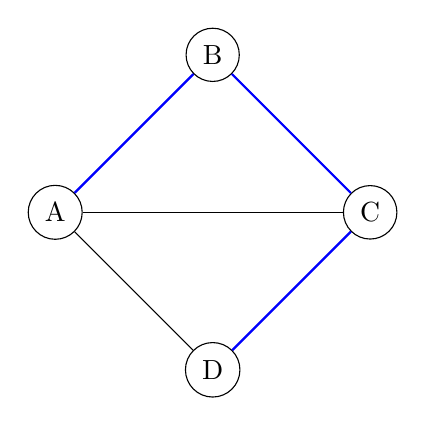
\begin{tikzpicture}
    % Define the vertices
    \node[draw, circle] (A) at (0, 0) {A};
    \node[draw, circle] (B) at (2, 2) {B};
    \node[draw, circle] (C) at (4, 0) {C};
    \node[draw, circle] (D) at (2, -2) {D};
    
    % Define the edges
    \draw (A) -- (B);
    \draw (B) -- (C);
    \draw (C) -- (D);
    \draw (A) -- (C);
    \draw (A) -- (D);
    
    % Highlight the Hamiltonian Path A-B-C-D
    \draw[blue, thick] (A) -- (B);
    \draw[blue, thick] (B) -- (C);
    \draw[blue, thick] (C) -- (D);
\end{tikzpicture}
\end{center}

For the directed graphs below, the graph on the left has a Hamiltonian Path from A to D, while the graph on the right does not have a Hamiltonian Path from A to D.

\begin{center}
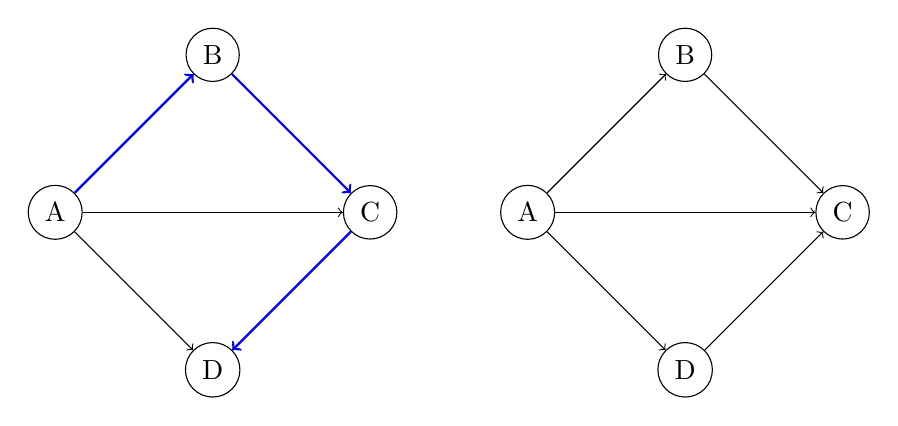
\begin{tikzpicture}
    % First graph with Hamiltonian Path
    \node[draw, circle] (A1) at (0, 0) {A};
    \node[draw, circle] (B1) at (2, 2) {B};
    \node[draw, circle] (C1) at (4, 0) {C};
    \node[draw, circle] (D1) at (2, -2) {D};
    
    \draw[->] (A1) -- (B1);
    \draw[->] (B1) -- (C1);
    \draw[->] (C1) -- (D1);
    \draw[->] (A1) -- (C1);
    \draw[->] (A1) -- (D1);
    
    \draw[blue, thick, ->] (A1) -- (B1);
    \draw[blue, thick, ->] (B1) -- (C1);
    \draw[blue, thick, ->] (C1) -- (D1);

    % Second graph without Hamiltonian Path
    \node[draw, circle] (A2) at (6, 0) {A};
    \node[draw, circle] (B2) at (8, 2) {B};
    \node[draw, circle] (C2) at (10, 0) {C};
    \node[draw, circle] (D2) at (8, -2) {D};
    
    \draw[->] (A2) -- (B2);
    \draw[->] (B2) -- (C2);
    \draw[->] (D2) -- (C2);
    \draw[->] (A2) -- (C2);
    \draw[->] (A2) -- (D2);

\end{tikzpicture}
\end{center}

We refer to the undirected version of this problem as \textbf{UHP} and the directed version as \textbf{DHP}.

\begin{questions}

    \question[3] Give a reduction from UHP to DHP.

    \ifsolutions\input{q1a-sol.tex}\fi

    \question[4] Prove the correctness of your reduction from UHP to DHP. That is, prove that the answer to your reduced DHP instance is YES if and only if the answer to UHP is YES. 

    \ifsolutions\input{q1b-sol.tex}\fi

    \question[7] Give a reduction from DHP to UHP. You \textbf{do not} need to prove the correctness of this reduction, but you should clearly explain the key components of your reduction and why they are there.

    \ifsolutions\input{q1c-sol.tex}\fi

%===============================
\section{Strategically Placed Krispy Kremes}

This SPKK problem is also in Tutorial 6. UBC Rec student leaders are planning their next fundraiser, and are seeking your help in identifying strategic locations to set up their stands of Krispy Kremes. They have a map showing $n$ locations of buildings and outdoor spots on campus. Their $k$ stands need to be set up in the outdoor spots. They want you to select $k$ spots such that the maximum distance from any of the $n$ locations to a stand is as small as possible.

An instance of the Strategically Placed Krispy Kremes decision problem (SPKK) has a set $V$ of size $n$, a subset $S$ of $V$, an integer $k$, $1\le k \le |S|$,  and a symmetric matrix $d[1..n][1..n]$, plus an additional nonnegative integer $b$. The problem is to determine if there is a subset $S' \subseteq S$ of size $k$, such that

\[
\max_{v \in V} \min_{s \in S'} \{ d[v][s] \;|\; s \in S' \} \le b.
\]

\begin{questions}
\question[8]
Provide a reduction from the Dominating Set problem to SPKK.
Briefly justify why the reduction is polynomial-time (one sentence is sufficient). Carefully explain why your reduction is correct (two paragraphs is sufficient).

 
  \ifsolutions\input{q1a-sol.tex}\fi
  \end{questions}


\end{questions}